\documentclass[ignorenonframetext,]{beamer}
\setbeamertemplate{caption}[numbered]
\setbeamertemplate{caption label separator}{: }
\setbeamercolor{caption name}{fg=normal text.fg}
\beamertemplatenavigationsymbolsempty
\usepackage{lmodern}
\usepackage{amssymb,amsmath}
\usepackage{ifxetex,ifluatex}
\usepackage{fixltx2e} % provides \textsubscript
\ifnum 0\ifxetex 1\fi\ifluatex 1\fi=0 % if pdftex
  \usepackage[T1]{fontenc}
  \usepackage[utf8]{inputenc}
\else % if luatex or xelatex
  \ifxetex
    \usepackage{mathspec}
  \else
    \usepackage{fontspec}
  \fi
  \defaultfontfeatures{Ligatures=TeX,Scale=MatchLowercase}
\fi
% use upquote if available, for straight quotes in verbatim environments
\IfFileExists{upquote.sty}{\usepackage{upquote}}{}
% use microtype if available
\IfFileExists{microtype.sty}{%
\usepackage{microtype}
\UseMicrotypeSet[protrusion]{basicmath} % disable protrusion for tt fonts
}{}
\newif\ifbibliography
\hypersetup{
            pdftitle={Week 03: Civil Wars},
            pdfauthor={Danilo Freire},
            pdfborder={0 0 0},
            breaklinks=true}
\urlstyle{same}  % don't use monospace font for urls
\usepackage{graphicx,grffile}
\makeatletter
\def\maxwidth{\ifdim\Gin@nat@width>\linewidth\linewidth\else\Gin@nat@width\fi}
\def\maxheight{\ifdim\Gin@nat@height>\textheight0.8\textheight\else\Gin@nat@height\fi}
\makeatother
% Scale images if necessary, so that they will not overflow the page
% margins by default, and it is still possible to overwrite the defaults
% using explicit options in \includegraphics[width, height, ...]{}
\setkeys{Gin}{width=\maxwidth,height=\maxheight,keepaspectratio}

% Prevent slide breaks in the middle of a paragraph:
\widowpenalties 1 10000
\raggedbottom

\AtBeginPart{
  \let\insertpartnumber\relax
  \let\partname\relax
  \frame{\partpage}
}
\AtBeginSection{
  \ifbibliography
  \else
    \let\insertsectionnumber\relax
    \let\sectionname\relax
    \frame{\sectionpage}
  \fi
}
\AtBeginSubsection{
  \let\insertsubsectionnumber\relax
  \let\subsectionname\relax
  \frame{\subsectionpage}
}

\setlength{\parindent}{0pt}
\setlength{\parskip}{6pt plus 2pt minus 1pt}
\setlength{\emergencystretch}{3em}  % prevent overfull lines
\providecommand{\tightlist}{%
  \setlength{\itemsep}{0pt}\setlength{\parskip}{0pt}}
\setcounter{secnumdepth}{0}

\title{Week 03: Civil Wars}
\subtitle{Causes of Civil Wars}
\author{Danilo Freire}
\date{24 September 2019}

\begin{document}
\frame{\titlepage}

\begin{frame}

\end{frame}

\begin{frame}{Last week we saw that\ldots{}}

.font150{[} * Civil wars are crucial events in world history

\begin{itemize}
\tightlist
\item
  They are hard to define:

  \begin{itemize}
  \tightlist
  \item
    Partisan bias (favour victims)
  \item
    Political bias (war is not politics)
  \item
    Urban bias (costly information, big narratives)
  \item
    Selection bias (overaggregation, lack of context) {]} ---
  \end{itemize}
\end{itemize}

\end{frame}

\begin{frame}{Last week we saw that\ldots{}}

.font150{[} * Violence is both an outcome and an instrument of civil
wars

\begin{itemize}
\item
  Even barbaric acts can be rational
\item
  Quantitative measures are somewhat arbitrary
\item
  PRIO/UCDP and ACLED

  \begin{itemize}
  \tightlist
  \item
    25/1000 annual battle-related deaths
  \item
    ``contested incompatibility over territory or government and one of
    the parties is the state'' {]} ---
  \end{itemize}
\end{itemize}

\end{frame}

\begin{frame}[fragile]{Last week we saw that\ldots{}}

.font150{[} * Three waves of civil war

\begin{verbatim}
- Cold War: class-based conflicts, peasant rebellions
- 1991-2003: ethnic conflicts 
- 2003-present: radical Islamism, but religion might not be the main cause
\end{verbatim}

\begin{block}{{]}}

class: inverse, center, middle

\end{block}

\end{frame}

\begin{frame}{Causes of civil war}

\end{frame}

\begin{frame}{Collier and Hoeffler (2004)}

.center{[}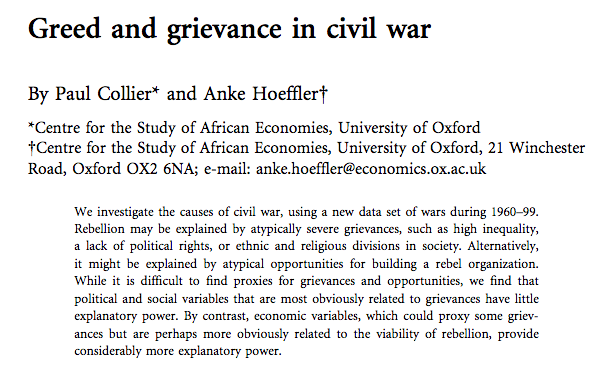
\includegraphics{ch00.png}{]}

\end{frame}

\begin{frame}{Collier and Hoeffler (2004)}

.font150{[} * C\&H argue political scientists put too much emphasis on
motivations (grievances)

\begin{itemize}
\item ~
  \subsection{Grievances are more or less constant, so why do civil wars
  break only at a specific point in
  time?{]}}\label{grievances-are-more-or-less-constant-so-why-do-civil-wars-break-only-at-a-specific-point-in-time}

  .font150{[}
\item
  \emph{Window of opportunity}: people rebel \emph{when they can}
\item
  Greed: atypical circumstances that can generate large returns
\item
  Yet they agree they cannot differentiate between \emph{opportunity}
  and \emph{viability} to express grievances {]} ---
\end{itemize}

\end{frame}

\begin{frame}{Proxies for opportunity}

.font150{[} * \textbf{Mineral resources}

\begin{itemize}
\item
  Ratio of primary exports to GDP
\item
  Relationship is non-linear
\item
  Countries with very low and very high ratios do not have civil wars
\item
  \textbf{Question}: why? {]} --
\end{itemize}

.font150{[} * Countries with few natural resources have nothing to loot
* Oil-rich countries can hold the country together by force * Those who
are above average are the best to loot{]} ---

\end{frame}

\begin{frame}{Proxies for opportunity}

.font150{[} * \textbf{Money from diasporas}

\begin{itemize}
\item
  E.g.: Tamil Tigers funded by American-resident Tamils
\item
  Proxied by \% of emigrants living in the US {]} ---
\end{itemize}

\end{frame}

\begin{frame}{Proxies for opportunity}

.font150{[} * \textbf{Funding from hostile governments}

\begin{itemize}
\tightlist
\item
  Examples:

  \begin{itemize}
  \tightlist
  \item
    Algerian civil war (rebels supported by USSR/ France by the US)
  \item
    Soviet-Afghan war (Sunni Mujahideen supported by US/PAK/CH, etc;
    Shia Mujahideen supported by Iran)
  \item
    Syrian civil war (a mess!) {]} ---
  \end{itemize}
\end{itemize}

\end{frame}

\begin{frame}{Proxies for opportunity}

.font150{[} * \textbf{Low cost of fighting}:

\begin{itemize}
\item
  \begin{enumerate}
  \def\labelenumi{\arabic{enumi})}
  \tightlist
  \item
    Income is low: GDP per capita
  \end{enumerate}
\item
  \begin{enumerate}
  \def\labelenumi{\arabic{enumi})}
  \setcounter{enumi}{1}
  \tightlist
  \item
    Weapons are cheap: previous wars
  \end{enumerate}
\item
  \begin{enumerate}
  \def\labelenumi{\arabic{enumi})}
  \setcounter{enumi}{2}
  \tightlist
  \item
    Government is weak: montainous terrain
  \end{enumerate}
\item
  \begin{enumerate}
  \def\labelenumi{\arabic{enumi})}
  \setcounter{enumi}{3}
  \tightlist
  \item
    Social cohesion: ethnic diversity {]} ---
  \end{enumerate}
\end{itemize}

\end{frame}

\begin{frame}{Proxies for grievances}

.font150{[} * Ethnic and religious hatred: ethnic fractionalisation

\begin{itemize}
\item
  Political repression: non-democracies
\item
  Political exclusion: ethnic dominance (majority group comprises
  45-90\% pop)
\item
  Economic inequality: Gini index, ratio top-to-bottom income {]} ---
\end{itemize}

\end{frame}

\begin{frame}{Opportunity model}

\begin{block}{.center{[}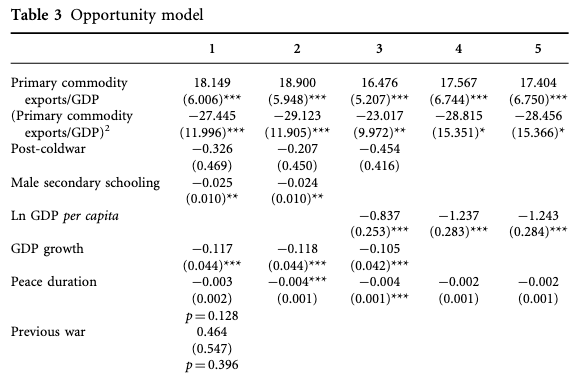
\includegraphics{ch01.png}{]}}

\end{block}

\end{frame}

\begin{frame}{Opportunity model}

\begin{block}{.center{[}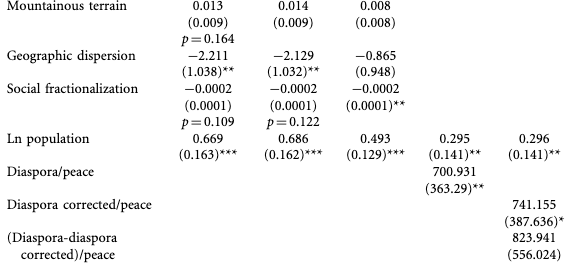
\includegraphics{ch02.png}{]}}

\end{block}

\end{frame}

\begin{frame}{Grievance model}

.font120{[}Drops economic variables from the model{]}

\begin{block}{.center{[}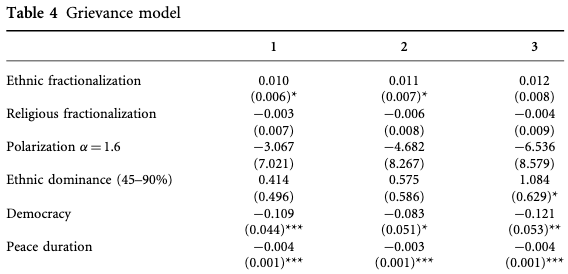
\includegraphics{ch03.png}{]}}

\end{block}

\end{frame}

\begin{frame}{Grievance model}

\begin{block}{.center{[}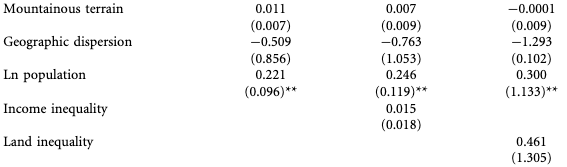
\includegraphics{ch04.png}{]}}

\end{block}

\end{frame}

\begin{frame}{Combined model}

\begin{block}{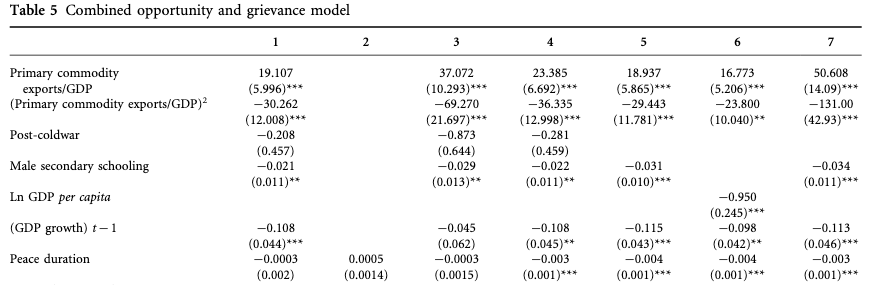
\includegraphics[width=1100px,height=400px]{ch05}}

\end{block}

\end{frame}

\begin{frame}{Combined model}

\begin{block}{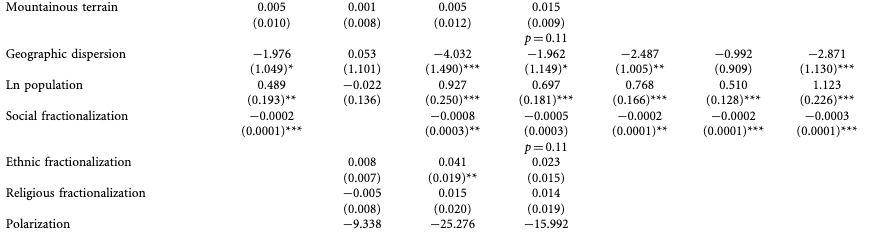
\includegraphics[width=1100px,height=400px]{ch06}}

\end{block}

\end{frame}

\begin{frame}{Combined model}

\begin{block}{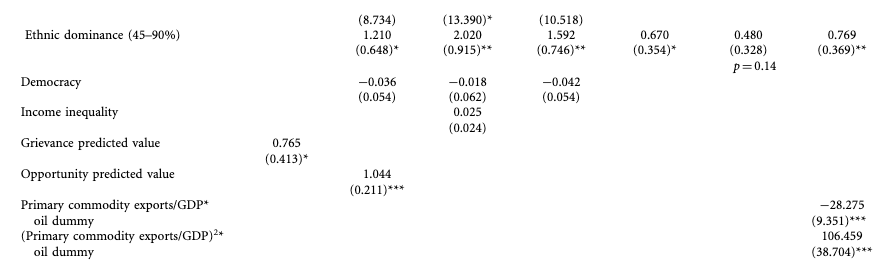
\includegraphics[width=1100px,height=400px]{ch07}}

\end{block}

\end{frame}

\begin{frame}{Interpretation}

.font150{[} * Factors that influence the opportunity for rebellion: -
Money from commodities - Diaspora - Low GDP - Dispersed population

\begin{itemize}
\item
  \emph{Find no evidence for grievance-based theories}
\item
  Only ethnic dominance has a positive effect
\item
  \textbf{Question}: what do you think? Is their explanation convincing?
  {]} ---
\end{itemize}

\end{frame}

\begin{frame}{Comments}

.font150{[} * No difference between rebels and criminals

\begin{itemize}
\item
  GDP, democracy, primary exports change very slowly over time\ldots{}
  what explains the conflict onset?
\item
  Urban bias: no mention of rural dynamics
\item
  Passive role of the state in the conflict
\item
  Crude proxies for greed and grievances {]} ---
\end{itemize}

\end{frame}

\begin{frame}{Fearon and Laitin (2003)}

.font150{[} * Most cited paper in political science in the last 15 years

\begin{itemize}
\item
  Remarkable data collection effort
\item
  Four main points:

  \begin{itemize}
  \tightlist
  \item
    The end of the Cold War \emph{did not} cause civil wars
  \item
    Controlling for income, ethnicity or religion doesn't matter
  \item
    Also find little support for grievance-based theories
  \item
    Factors that explain \emph{insurgency} are the most relevant
  \end{itemize}
\item
  Different from C\&H, F\&L argue that low GDP proxies for \emph{state
  capacity} {]} ---
\end{itemize}

\end{frame}

\begin{frame}{Data}

.font150{[} * Conflicts that kill at least 1,000 people, at least 100
per year, rebels or government forces

\begin{itemize}
\item
  Include colonial wars
\item
  F\&L are cautious about their data on empires
\item
  They analyse the data both including and excluding colonial wars {]}
  ---
\end{itemize}

\end{frame}

\begin{frame}{Conflicts over time}

\begin{block}{.center{[}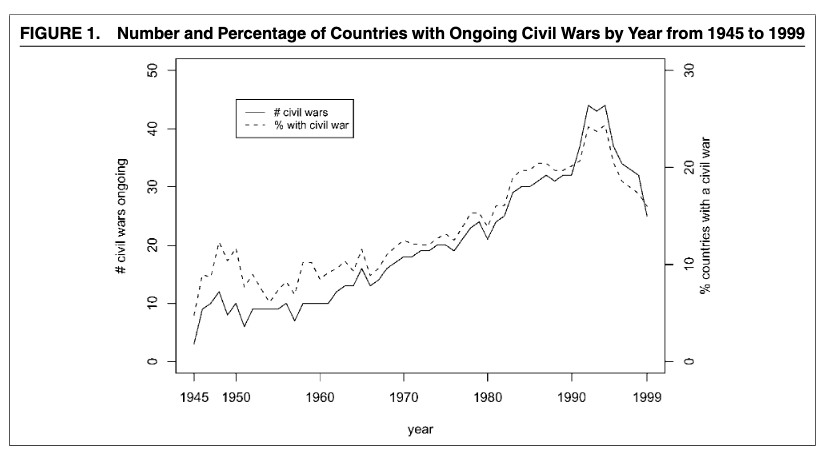
\includegraphics{fearon01.png}{]}}

\end{block}

\end{frame}

\begin{frame}{Ethnicity and conflict}

.font150{[} * They critique the idea of ``clash of civilisations''

\begin{itemize}
\item
  Deep-rooted ethnic grievances are not enough to explain civil war
  onset
\item
  Sceptical of ``modernisation theory'': limits to upward mobility cause
  people to revolt
\item
  Question that discrimination (ethnic of economic favoritism to other
  groups) leads to inequality {]} ---
\end{itemize}

\end{frame}

\begin{frame}{Insurgencies}

.font150{[} * Focus on small guerrilla wars

\begin{itemize}
\item
  Guerrilla groups are weak compared to the government
\item
  Factors that facilitate rebel group survival are very important

  \begin{itemize}
  \tightlist
  \item
    Montainous terrain (hideouts)
  \item
    Local knowledge
  \item
    Rural base
  \item
    Weak state governance {]} ---
  \end{itemize}
\end{itemize}

\end{frame}

\begin{frame}{Pred. probabilities: income and ethnicity}

\begin{block}{.center{[}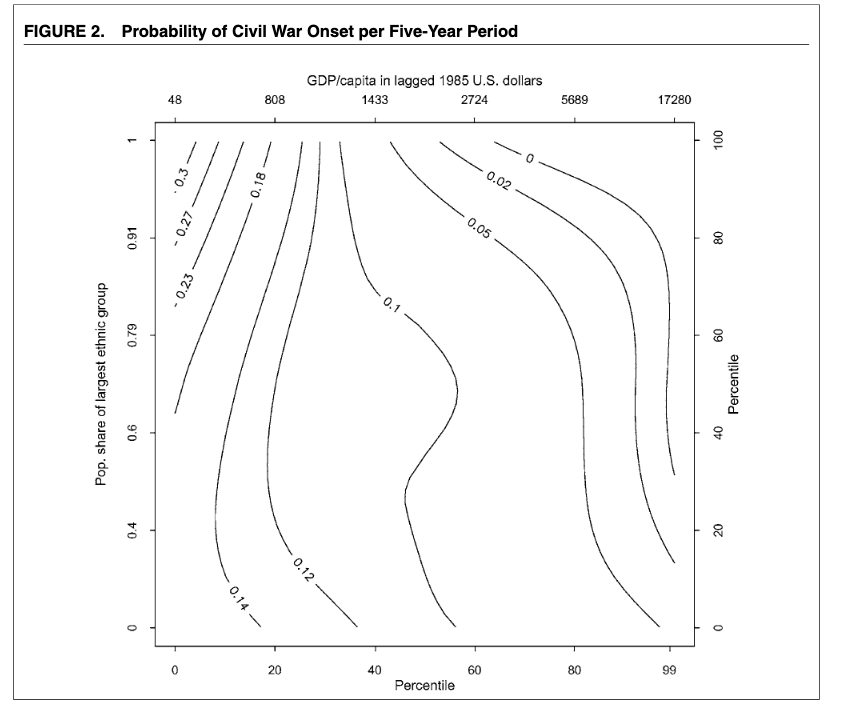
\includegraphics{fearon02.png}{]}}

\end{block}

\end{frame}

\begin{frame}{Main results}

\begin{block}{.center{[}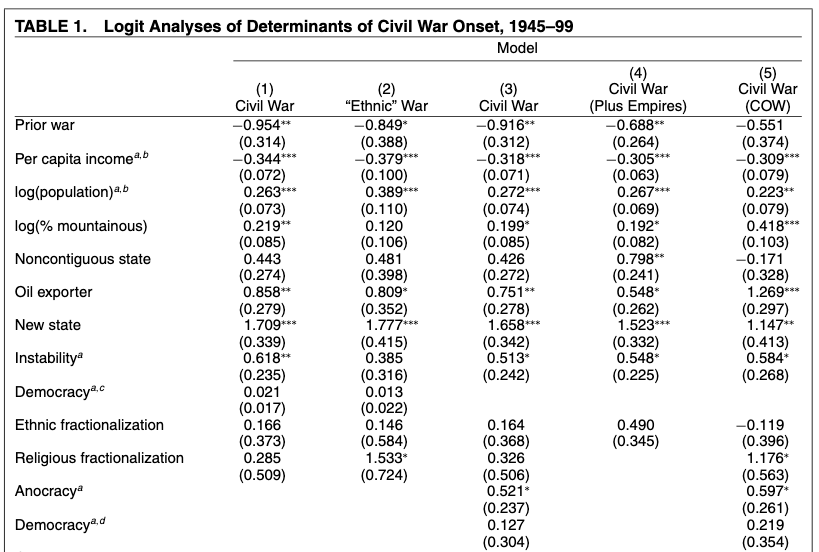
\includegraphics{fearon03.png}{]}}

\end{block}

\end{frame}

\begin{frame}{Discussion}

.font140{[} * The high number of civil wars in the 1990s is the result
of accumulation of previous conflicts, not the end of the Cold War

\begin{itemize}
\item
  Ethnicities and grievances do not explain why internal wars occur
\item
  Factors that favour \emph{insurgency} do: state weakness, low GDP,
  instability, and large population
\item
  Practical implications:

  \begin{itemize}
  \tightlist
  \item
    Promoting democracy abroad doesn't work
  \item
    Cultural dialogue doesn't work either
  \item
    Little foreign states can do: GDP, state capacity take time {]} ---
  \end{itemize}
\end{itemize}

\end{frame}

\begin{frame}{Comments on C\&H and F\&L}

.font150{[} * C\&H: \emph{homo oeconomicus} goes to war

\begin{itemize}
\item
  Rebels are essentially criminals: profits from looting
\item
  \textbf{Question}: natural/lootable resources can fuel grievances too,
  can't they? {]} --
\end{itemize}

.font150{[} * Resource-rich countries might have higher inequality,
forced migrations, trade shocks, etc

\begin{itemize}
\tightlist
\item
  Diasporas can also provide welfare to local communities and therefore
  \emph{reduce} the likelihood of conflict {]} ---
\end{itemize}

\end{frame}

\begin{frame}{Comments on C\&H and F\&L}

.font150{[} * F\&L: unclear which aspect of state capacity decreases
civil war risk: Inclusive institutions, shared power, armed forces,
economic redistribution?

\begin{itemize}
\item
  Impossible to adjudicate between their theory (state capacity, proxied
  by GDP per capita) and C\&H's (lootable resources, proxied by\ldots{}.
  GDP per capita!)
\item
  As with C\&H, national-level data obscures important within-country
  dynamics {]} ---
\end{itemize}

class: inverse, center, middle

\end{frame}

\begin{frame}{Questions?}

\end{frame}

\begin{frame}{Wimmer et al (2009)}

.font150{[} * Ethnicity \emph{does} play a role in civil war outbreaks

\begin{itemize}
\item
  Qualify previous literature
\item
  Offer better data on ethnic groups
\item
  Establish new mechanisms that link group grievances to conflicts
\item
  Focus on political dynamics of ethnic exclusion and competition {]}
  ---
\end{itemize}

\end{frame}

\begin{frame}{Institutionalist, configurational theory}

.font150{[} * \textbf{Institutionalist}: political structures create
incentives for players to act strategically

\begin{itemize}
\item
  \textbf{Configurational}: the same institution provides different
  incentives according to the distribution of power
\item
  Ethnicity matters \emph{because the nation state uses it for
  legitimacy}
\item
  Politicians have incentives to favour their co-ethnics
\item
  Ethnic favouritism is more likely in poor, young states (who need more
  legitimacy) {]} ---
\end{itemize}

\end{frame}

\begin{frame}{Institutionalist, configurational theory}

\begin{block}{.center{[}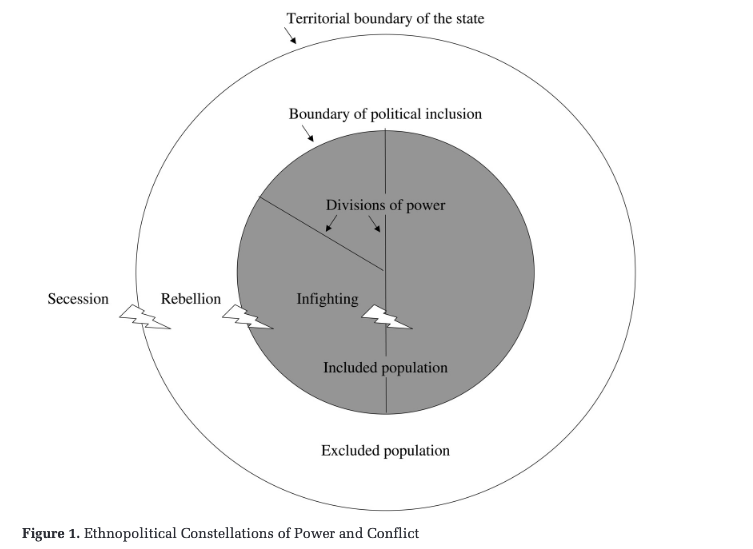
\includegraphics{wimmer01.png}{]}}

\end{block}

\end{frame}

\begin{frame}{Three types of ethnic conflict}

.font150{[} * \textbf{Secession}: changing the territorial boundaries of
a polity and can be pursued by both excluded and included groups

\begin{itemize}
\item
  \textbf{Rebellion}: excluded segments of a population fight to shift
  the boundaries of inclusion
\item
  \textbf{Infighting}: elite disputes for the spoils of government
\item
  Predictions:

  \begin{itemize}
  \tightlist
  \item
    ethnic exclusion breeds conflict
  \item
    more power-sharing increase conflict (coalitions)
  \item
    large states and those under indirect rule rebel more {]} ---
  \end{itemize}
\end{itemize}

\end{frame}

\begin{frame}{Results}

\begin{block}{.center{[}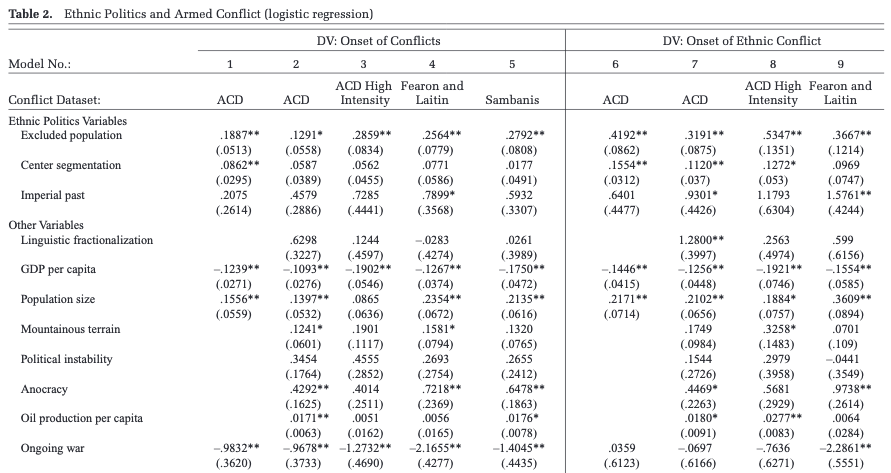
\includegraphics{wimmer02.png}{]}}

\end{block}

\end{frame}

\begin{frame}{Results}

\begin{block}{.center{[}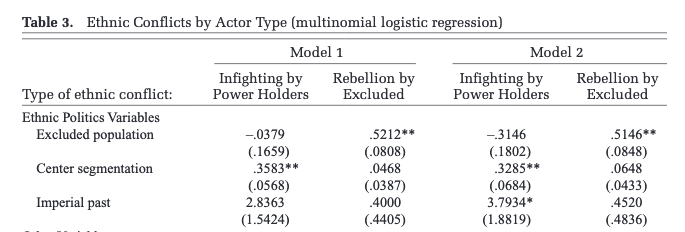
\includegraphics{wimmer03.png}{]}}

\end{block}

\end{frame}

\begin{frame}{Results}

\begin{block}{.center{[}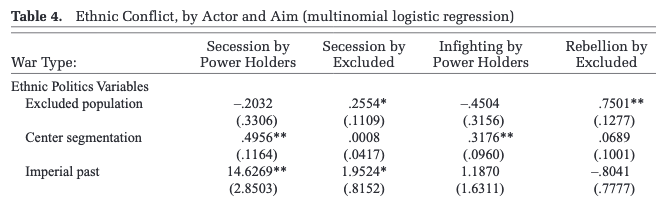
\includegraphics{wimmer04.png}{]}}

\end{block}

\end{frame}

\begin{frame}{Conclusion}

.font150{[} * ``The likelihood of armed confrontation increases as the
center of power becomes more ethnically segmented and as greater
proportions of a states population are excluded from power because of
their ethnic background''

\begin{itemize}
\item
  ``These conflicts are even more likely in incoherent states where the
  population is not accustomed to direct rule by the political center''
\item
  ``Ethnicity is not an aim in itself, but the organizational means
  through which individuals struggle to gain access to state power'' {]}
  ---
\end{itemize}

\end{frame}

\begin{frame}{Comments on Wimmer et al}

.font150{[} * Good idea to focus on ethnicity and power dynamics

\begin{itemize}
\item
  However, still treats ethnicity as a fixed category
\item
  Ethnicity and conflict can be endogenous
\item
  Urban bias, maybe? {]} ---
\end{itemize}

class: inverse, center, middle

\end{frame}

\begin{frame}{Questions?}

\end{frame}

\begin{frame}{Kalyvas and Balcells (2010)}

.font150{[} * Does systemic factors play a role in civil war dynamics?

\begin{itemize}
\item
  More specifically, what is the role of the international system in
  civil wars?
\item
  ``Technologies of rebellion'': ways that civil conflicts are fought
\item
  Disaggregating the types of conflict
\item
  The end of the Cold War caused a decline in irregular wars {]} ---
\end{itemize}

\end{frame}

\begin{frame}{Technologies of rebellion}

.font150{[} * \textbf{Irregular warfare}: guerrillas

\begin{itemize}
\item
  \textbf{Conventional warfare}: army and rebels have similar power
\item
  \textbf{Symmetric non-conventional (SNC) warfare}: states
  unable/unwilling to fight (``primitive'' wars) {]} ---
\end{itemize}

\end{frame}

\begin{frame}{The puzzle of the Cold War}

.font150{[} * Civil wars were understood as proxy wars

\begin{itemize}
\tightlist
\item
  End of the Cold War brought changes to the int'l system:

  \begin{itemize}
  \tightlist
  \item
    End of multiethnic states
  \item
    Emergence of new states
  \item
    Cheap weapons from the former USSR
  \item
    Weakening of client states
  \item
    No legitimising principle to the state (link with Wimmer et al.)
  \end{itemize}
\item
  Contest F\&L's results that the Cold War has no effect {]} ---
\end{itemize}

\end{frame}

\begin{frame}{Technologies of rebellion}

\begin{block}{.center{[}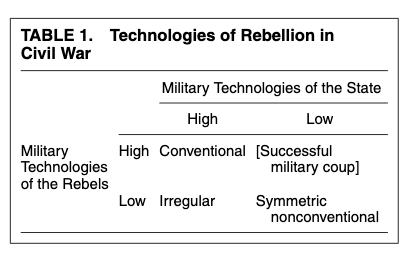
\includegraphics{kb01.png}{]}}

\end{block}

\end{frame}

\begin{frame}{Summary statistics}

\begin{block}{.center{[}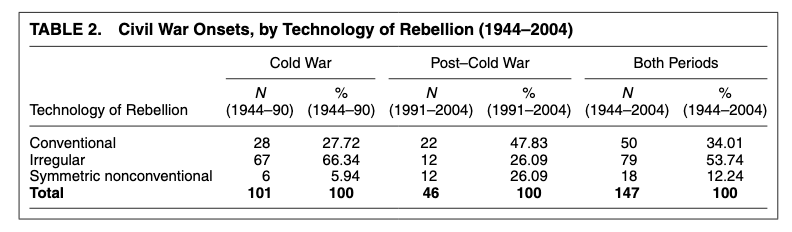
\includegraphics{kb02.png}{]}}

\end{block}

\end{frame}

\begin{frame}{Main results}

.font150{[} * 1 for conventional wars, 2 for irregular wars, and 3 for
SNC wars. {]}

\begin{block}{.center{[}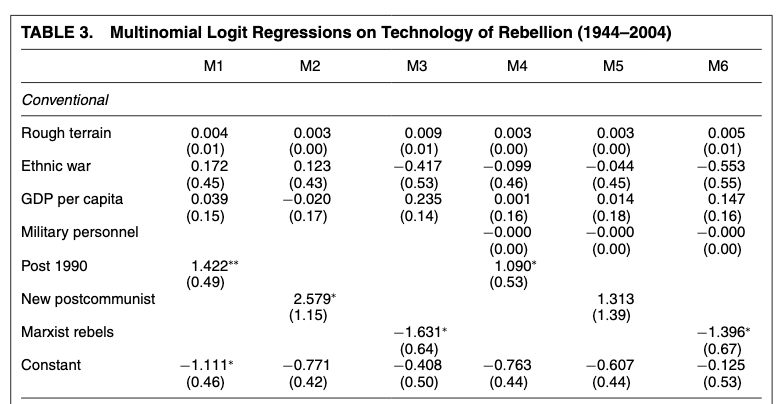
\includegraphics{kb03.png}{]}}

\end{block}

\end{frame}

\begin{frame}{Main results}

\begin{block}{.center{[}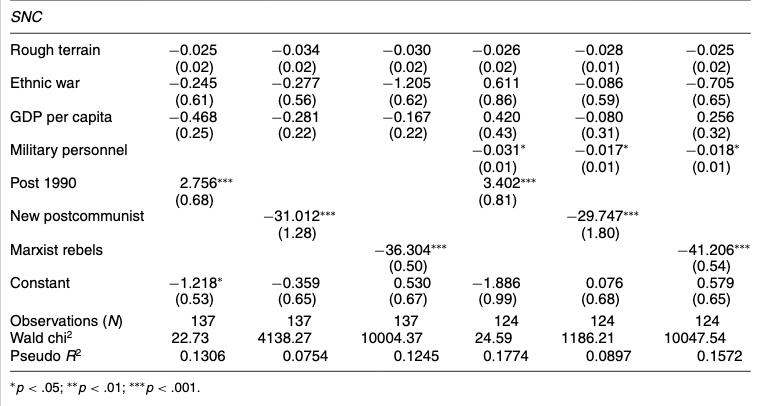
\includegraphics{kb04.png}{]}}

\end{block}

\end{frame}

\begin{frame}{Discussion}

.font150{[} * Indeed the ``technologies of rebellion'' had been
overlooked

\begin{itemize}
\item
  However, the model doesn't seem very convincing
\item
  Almost nothing is significant; bad control variables
\item
  No testing of any mechanism:

  \begin{itemize}
  \tightlist
  \item
    Material support
  \item
    Ideological cohesion
  \item
    Access to weapons
  \end{itemize}
\item
  SNC is a poorly-defined category {]} ---
\end{itemize}

\end{frame}

\begin{frame}{Ward et al (2010)}

.font150{[} * Statistical models explain what has already
happened\ldots{}

\begin{itemize}
\item
  How useful are they to predict \emph{what might happen in the future}?
\item
  In-sample vs out-of-sample testing
\item
  Limitations of statistical models
\item
  Possible means for testing the validity of a theory: see how it
  performs with new data {]} ---
\end{itemize}

\end{frame}

\begin{frame}{Problems of statistical significance}

.font140{[} * False positives and false negatives - Every probability
above 0.5 is considered positive in the model - There is \emph{nothing}
special about that number

\begin{itemize}
\tightlist
\item
  \textbf{Question}:

  \begin{itemize}
  \tightlist
  \item
    You are the leader of your country and you see that country X has
    50\% chance of going to war next year. If you are right, a civil war
    can be averted. \emph{But if you are wrong}, you will invade another
    country, your citizens will die, and conflict might spread. What
    probability would make \emph{you} go to war? {]} ---
  \end{itemize}
\end{itemize}

\end{frame}

\begin{frame}{Statistical vs predictive power}

\begin{block}{.center{[}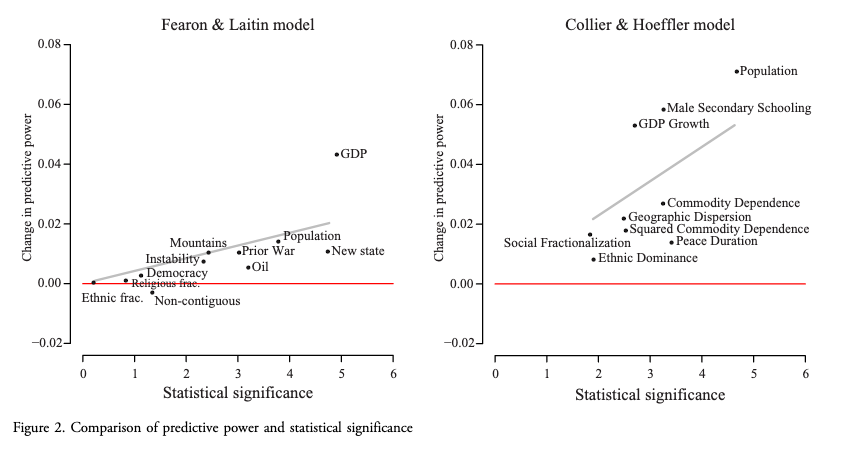
\includegraphics{ward01.png}{]}}

\end{block}

\end{frame}

\begin{frame}{Discussion}

.font150{[} * Variables that are statistically significant have little
predictive power

\begin{itemize}
\item
  How can we use these models to prepare for new conflicts?
\item
  Factors that explain previous civil wars may not explain future ones
\item
  Prediction can help us build more robust (although not necessarily
  more efficient) models for civil war prevention {]} ---
\end{itemize}

class: inverse, center, middle

\end{frame}

\begin{frame}{Questions?}

\end{frame}

\begin{frame}{Brief summary}

.font150{[} * Civil wars happen in poor, weak states

\begin{itemize}
\item
  Windows of opportunity are more important than old grievances
\item
  Ethnic rivalries can lead to civil war outbreak, but under certain
  conditions
\item
  The Cold War has changed the way civil wars are fought
\item
  Many of the variables we know explain \emph{past} wars, but can they
  explain future ones? {]} ---
\end{itemize}

\end{frame}

\begin{frame}{Similar analysis}

\begin{block}{.center{[}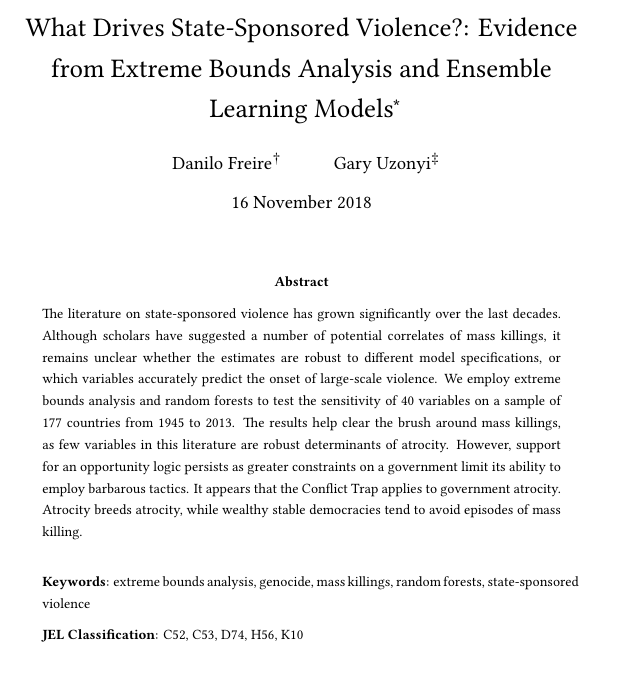
\includegraphics{freire01.png}{]}}

\end{block}

\end{frame}

\begin{frame}{To conclude}

.center{[}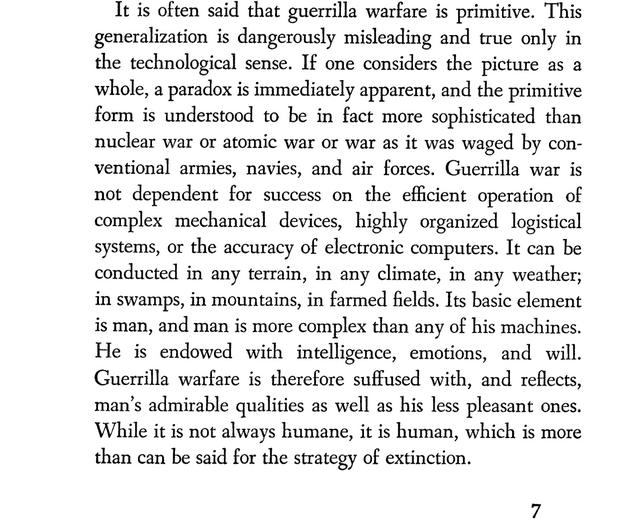
\includegraphics{griffith.png}{]}

\begin{block}{.center{[}Source:
\href{https://books.google.com/books?id=jKoqAwAAQBAJ\&lpg=PA7\&dq=griffith\%20\%22its\%20basic\%20element\%20is\%22\&pg=PA7\#v=onepage\&q\&f=false}{Griffith,
S. B. - Introduction to Mao Zedong's \emph{On Guerrilla Warfare}
(1961)}{]}}

class: inverse, center, middle

\end{block}

\end{frame}

\begin{frame}{See you next week!}

\end{frame}

\end{document}
